% $Header: /Users/joseph/Documents/LaTeX/beamer/solutions/conference-talks/conference-ornate-20min.en.tex,v 90e850259b8b 2007/01/28 20:48:30 tantau $
\RequirePackage{filecontents}
\begin{filecontents*}{seminar.bib}
@book{test,
author={John Smith},
title={A book},
publisher={Puplisher},
year={1742},
}
\end{filecontents*}
\documentclass{beamer}
\usepackage{graphicx}

\usepackage{latexsym}		% to get LASY symbols
\usepackage{epsfig}		% to insert PostScript figures
\usepackage{rotating}		% for sideways tables/figures
\usepackage{eufrak}
\usepackage{natbib}
\def\newblock{\hskip .11em plus .33em minus .07em}

% This file is a solution template for:

% - Talk at a conference/colloquium.
% - Talk length is about 20min.
% - Style is ornate.



% Copyright 2004 by Till Tantau <tantau@users.sourceforge.net>.
%
% In principle, this file can be redistributed and/or modified under
% the terms of the GNU Public License, version 2.
%
% However, this file is supposed to be a template to be modified
% for your own needs. For this reason, if you use this file as a
% template and not specifically distribute it as part of a another
% package/program, I grant the extra permission to freely copy and
% modify this file as you see fit and even to delete this copyright
% notice. 


\mode<presentation>
{
  \usetheme{Madrid}
  % or ...

  \setbeamercovered{transparent}
  % or whatever (possibly just delete it)
}


\usepackage[english]{babel}
% or whatever

\usepackage[latin1]{inputenc}
% or whatever

\usepackage{times}
\usepackage[T1]{fontenc}
% Or whatever. Note that the encoding and the font should match. If T1
% does not look nice, try deleting the line with the fontenc.


\title[AGRIMOBILE] % (optional, use only with long paper titles)
{AGRIMOBILE}
%
%\subtitle
%{Include Only If Paper Has a Subtitle}

\author[Group Number IV\\Group Members] % (optional, use only with lots of authors)
{Group Number IV\\Group Members}
% - Give the names in the same order as the appear in the paper.
% - Use the \inst{?} command only if the authors have different
%   affiliation.

\institute[MES College of Engineering] % (optional, but mostly needed)
{
 
  Amrutha K .V.-14BCS12163\\Neethu C .P.-14BCS12164\\Sreelakshmi T .G.-14BCS12165\\Thahsin P.-13BCS11154\\Suniya C .T.-14BCS12166
 \\Computer Science \& Engineering\\
  Guide: Mr.Sherikh K .K.(Asst.prof.)}
% - Use the \inst command only if there are several affiliations.
% - Keep it simple, no one is interested in your street address.

%\date[CFP 2003] % (optional, should be abbreviation of conference name)
%{Conference on Fabulous Presentations, 2003}
% - Either use conference name or its abbreviation.
% - Not really informative to the audience, more for people (including
%   yourself) who are reading the slides online

\subject{Theoretical Computer Science}
% the beginning of each subsection:

\AtBeginSubsection[]
{
	
	\tableofcontents[currentsection,currentsubsection]

 
  \end{frame}
}


% If you wish to uncover everything in a step-wise fashion, uncomment
% the following command: 

%\beamerdefaultoverlayspecification{<+->}


\begin{document}

\begin{frame}
  \titlepage
 \end{frame}

%\begin{frame}{Outline}
 % \tableofcontents
  % You might wish to add the option [pausesections]
%\end{frame}


% Structuring a talk is a difficult task and the following structure
% may not be suitable. Here are some rules that apply for this
% solution: 

% - Exactly two or three sections (other than the summary).
% - At *most* three subsections per section.
% - Talk about 30s to 2min per frame. So there should be between about
%   15 and 30 frames, all told.

% - A conference audience is likely to know very little of what you
%   are going to talk about. So *simplify*!
% - In a 20min talk, getting the main ideas across is hard
%   enough. Leave out details, even if it means being less precise than
%   you think necessary.
% - If you omit details that are vital to the proof/implementation,
%   just say so once. Everybody will be happy with that.

\subsection{INTRODUCTION}
\begin{frame}{INTRODUCTION}
   \begin{itemize}
    
   	\item Agriculture, the backbone of Indian economy.
   	\item Agrimobile provide relevant agriculture services for unorganized sector.
   	\item Information related to crop production and protection.
   	\item Doubt clearance and discussion 
   	\item Online purchasing .
   	\item Selling.
   	\end{itemize}
   	\end{frame} 
   	 
\begin{frame}{INTRODUCTION(Cond...)}
	\begin{itemize}
   	\item App developed for the members in FPO.
   	\item  FPO is one initiatives taken by the Department of Agriculture.
   	\item Collaborated with Krishi Vigyan Kendra, Thavanur.
   	\item Financial and technical advices are the major activities of FPO.
   \end{itemize}
 \end{frame}  

\subsection{ABSTRACT}
\begin{frame}{ABSTRACT}
   \begin{itemize}
  \item Android application.
  \item Useful for farmers & agricultural institutes.
  \item Collecting information and suggest suitable crops.
  \item Social networking group for share experiences and knowledge.
  \item Add their vegetables along with its price.  
  \item Purchase the vegetable with suitable prices.
  \end{itemize}
  \end{frame}
  
  \subsection{EXISTING SYSTEM}
  \begin{frame}{EXISTING SYSTEM}
  \begin{itemize}
  \item Most agriculture apps deals with huge commodity and people.
  \item Problem of control and coordinate.
  \item Lack of a proper marketing channel distress sale.
  \item Wastage of products.
  \item Production of some crops exceeding and some crops below the requirement.
  \end{itemize}
  \end{frame}
    
  \subsection{LITERATURE SURVEY}
  \begin{frame}{LITERATURE SURVEY}
  \begin{itemize}
  \item 2015 IEEE Technological Innovation in ICT for Agriculture and Rural Development (TIAR).
  \item Providing Smart Agricultural solutions to farmers for better yielding using IoT.
  \item  Mobile information system for small-scale rural farmers.
  \end{itemize}
  \end{frame}
  
  \subsection{2015 IEEE Technological Innovation in ICT for Agriculture and Rural Development (TIAR)}
  \begin{frame}{2015 IEEE Technological Innovation in ICT for Agriculture and Rural Development (TIAR)}
  \begin{itemize}
  \item 
  \item 
  \item 
  \end{itemize}
  \end{frame}
  
  \subsection{Providing Smart Agricultural solutions to farmers for better yielding using IoT.}
  \begin{frame}{Providing Smart Agricultural solutions to farmers for better yielding using IoT.}
  \begin{itemize}
  \item The field of Cloud computing is helping in leaps and bounds to improvise our age old business - Agriculture.
  \item Sensors to tools that observe data from agricultural field images and from human actors on the ground.
\item Accurately feed the data into repositories along with their location as GPS co-ordinates.
\item Sensors are now able to detect the position of water sources in a subject that is being investigated.
\end{itemize}
 \end{frame}
\begin{frame}{Providing Smart Agricultural solutions to farmers for better yielding using IoT.(Cond...)}
  \begin{itemize}
\item  One of the answer to these types of problems is to help the farmers using modernization techniques.
\item Combining the advantages of the major characteristics of emerging technologies such as Internet of Things(IoT) and Web Services. 
\item Combination of IoT and cloud computing that promotes the fast development of agricultural modernization.
\item Smart solution for agriculture and efficiently solve the issues related to farmers.
  \end{itemize}
  \end{frame}
  
  \subsection{Mobile information system for small-scale rural farmers}
  \begin{frame}{Mobile information system for small-scale rural farmers}
  \begin{itemize}
  \item Ethiopia Commodity Exchange (ECX disseminating market information to small-scale farmers and market actors through mobile-based market information systems (MKIS). 
  \item 
\item 
\item 
\end{itemize}
 \end{frame}
 
 \subsection{SYSTEM DESIGN}
  \begin{frame}{SYSTEM DESIGN}
  \begin{itemize}
  \item  
  \item 
  \item 
  \item 
\end{itemize}
 \end{frame}
  
 
 \subsection{MODULE DESCRIPTION}
\begin{frame}{MODULE DESCRIPTION}
   \begin{enumerate}
  \item Farmers module
  \begin{itemize}
   \item Doubt Clearance.
  \item Fertilizers/pesticides information.
  \item Discussion.
  \item Purchasing & marketing.
  \end{itemize}
 
  \item Customers module.
  \begin{itemize}
  \item Ordering.
  \item Purchasing.
   \end{itemize}
  \end{enumerate}
  \end{frame}
  
  
\subsection{DATA FLOW DIAGRAM}
\begin{frame}{DATA FLOW DIAGRAM}
   \begin{itemize}
  \item User registration
  \begin{figure}[ht!]
    \centering
    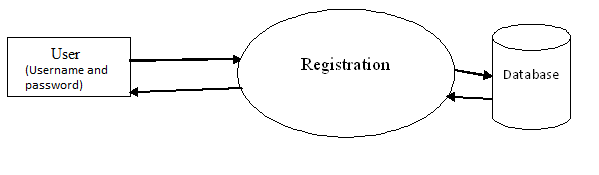
\includegraphics[width=10cm]{login1.png}
    
    \label{fig:pc control reg}
\end{figure}

  \item User login.
   
   \begin{figure}[ht!]
    \centering
    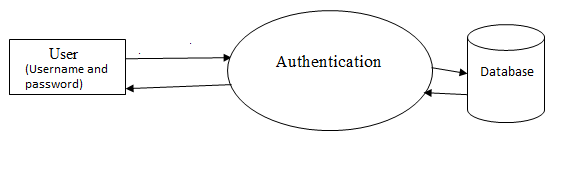
\includegraphics[width=10cm]{login2.png}
    
    \label{fig:pc control login}
\end{figure}
 
\end{itemize}

 \end{frame}

\begin{frame}{DATA FLOW DIAGRAM(Cont...)}
   \begin{itemize}
  \item Remote desktop access
  \begin{figure}[ht!]
    \centering
    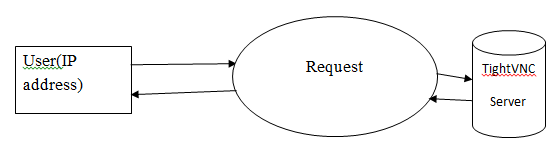
\includegraphics[width=10cm]{f3.png}
    \label{fig:pc control desk}
\end{figure}

  \item Power options
   
   \begin{figure}[ht!]
    \centering
    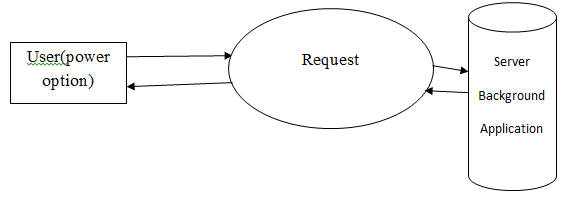
\includegraphics[width=10cm]{power1.png}    
    \label{fig:pc control power}
\end{figure}
\end{itemize}
 \end{frame}
 
 \begin{frame}{DATA FLOW DIAGRAM(Cont...)}
   \begin{itemize}
  \item Send message
  \begin{figure}[ht!]
    \centering
    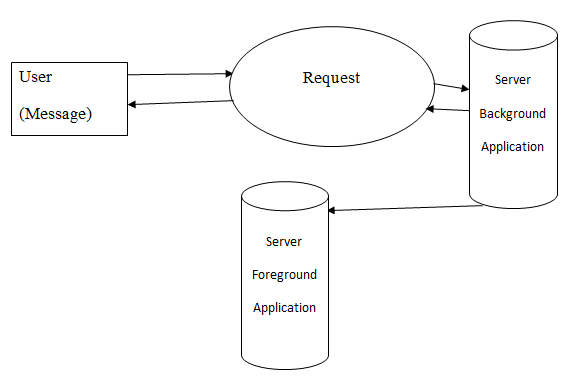
\includegraphics[width=10cm]{send1.png}   
    \label{fig:pc control send}
\end{figure}
\end{itemize}
\end{frame}

  
\subsection{DESIGN}
\begin{frame}{DESIGN}
\begin{itemize}
  	\item Screen shots  
   \begin{itemize}
  	\item Launcher 
 	 \begin{figure}[ht!]
     \centering
    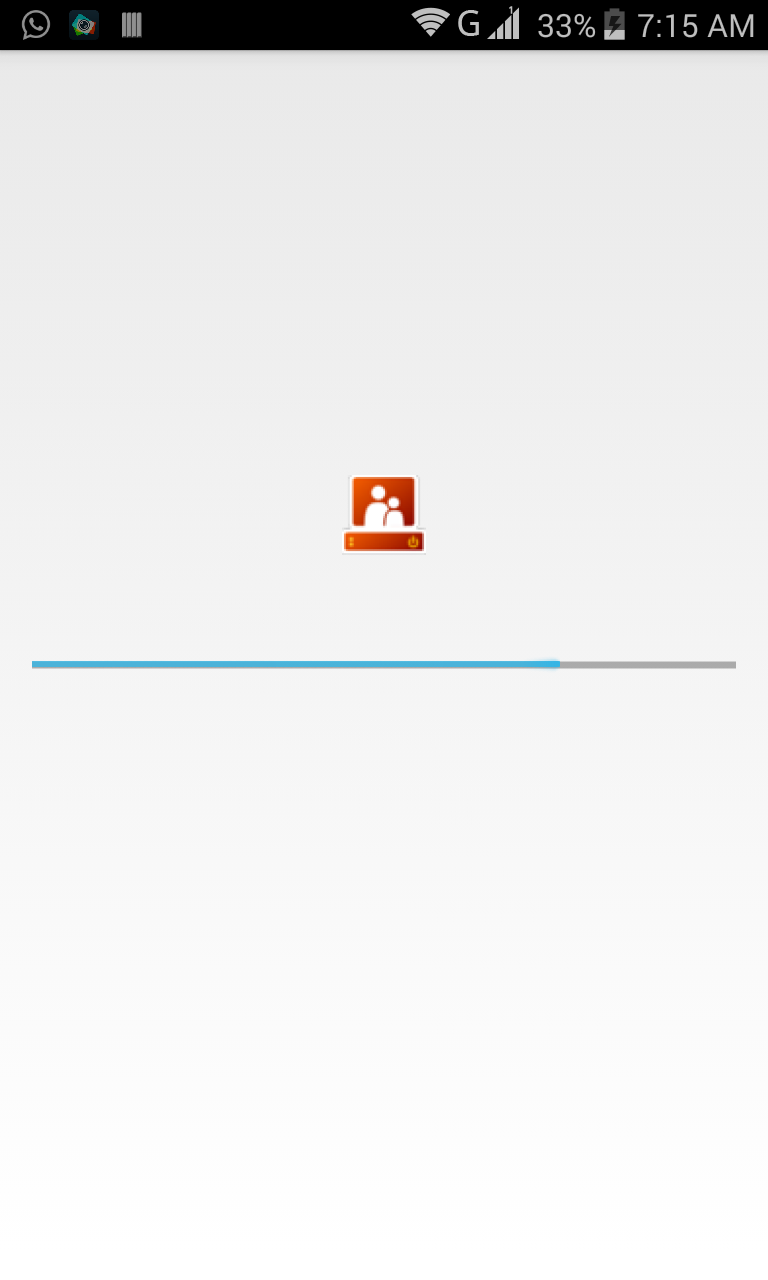
\includegraphics[width=4cm]{launch.png}
    
    \label{fig:pc control launch}
\end{figure}
\end{itemize}
\end{itemize}
 \end{frame} 

\begin{frame}{DESIGN(Cont...)}  
   \begin{itemize}
  	\item Terms and Conditions 
 	 \begin{figure}[ht!]
     \centering
    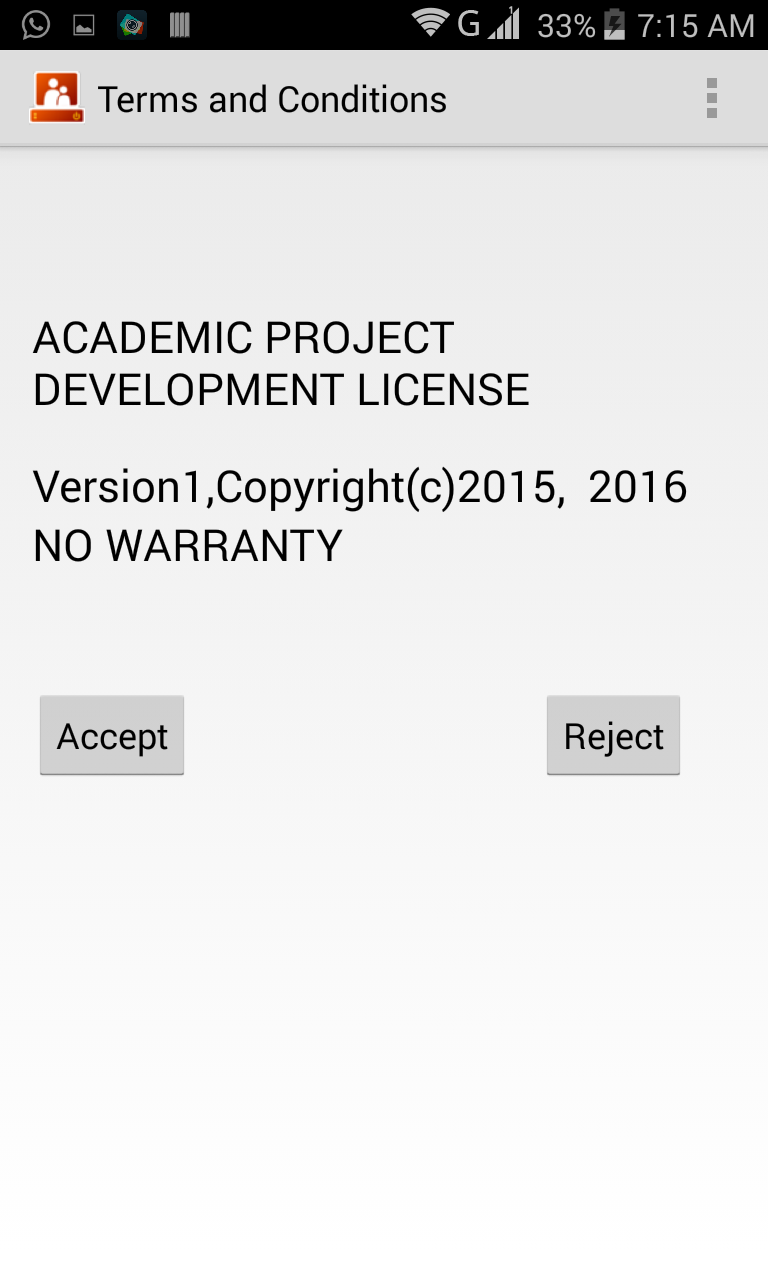
\includegraphics[width=4cm]{terms.png}
    \label{fig:pc control login}
\end{figure}
   \end{itemize}
 \end{frame} 
 
 \begin{frame}{DESIGN(Cont...)}  
   \begin{itemize}
  	\item User Registration 
 	 \begin{figure}[ht!]
     \centering
    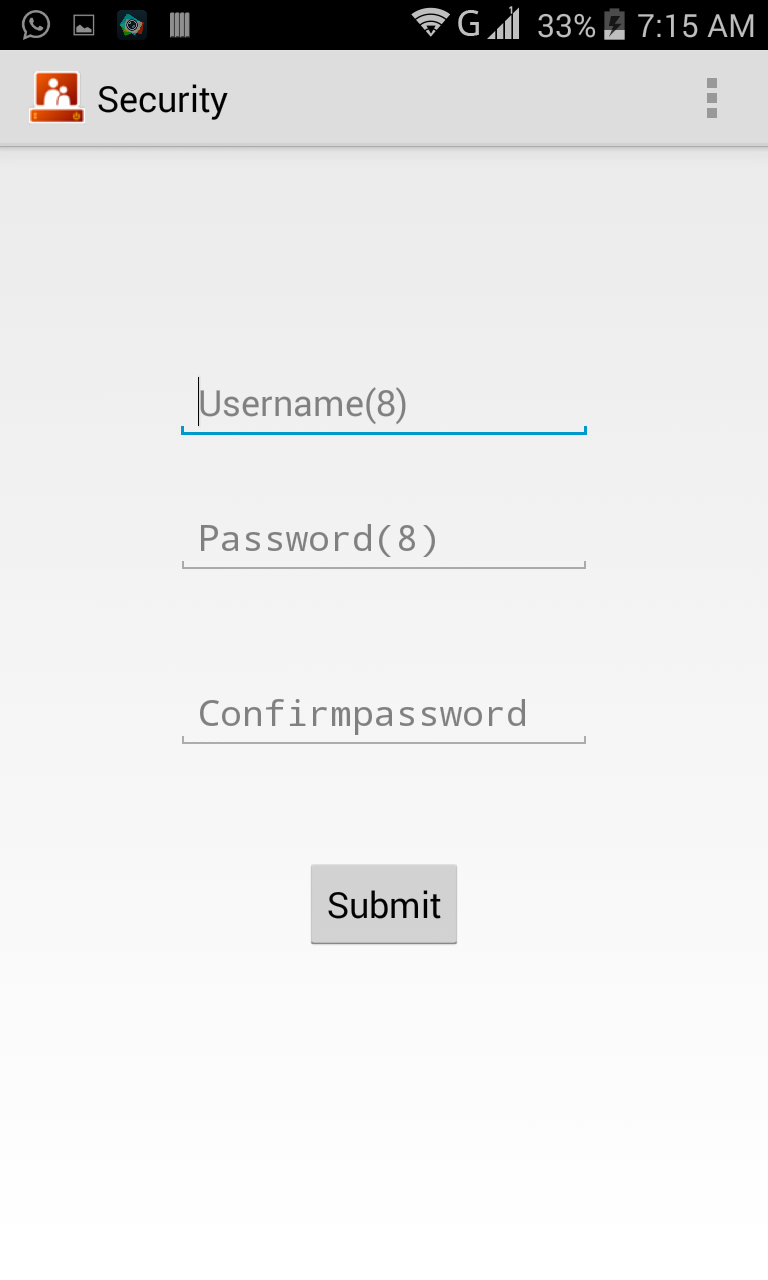
\includegraphics[width=4cm]{reg.png}
    \label{fig:pc control window}
\end{figure}
   \end{itemize}
 \end{frame} 
 
 \begin{frame}{DESIGN(Cont...)}  
   \begin{itemize}
  	\item User Login 
 	 \begin{figure}[ht!]
     \centering
    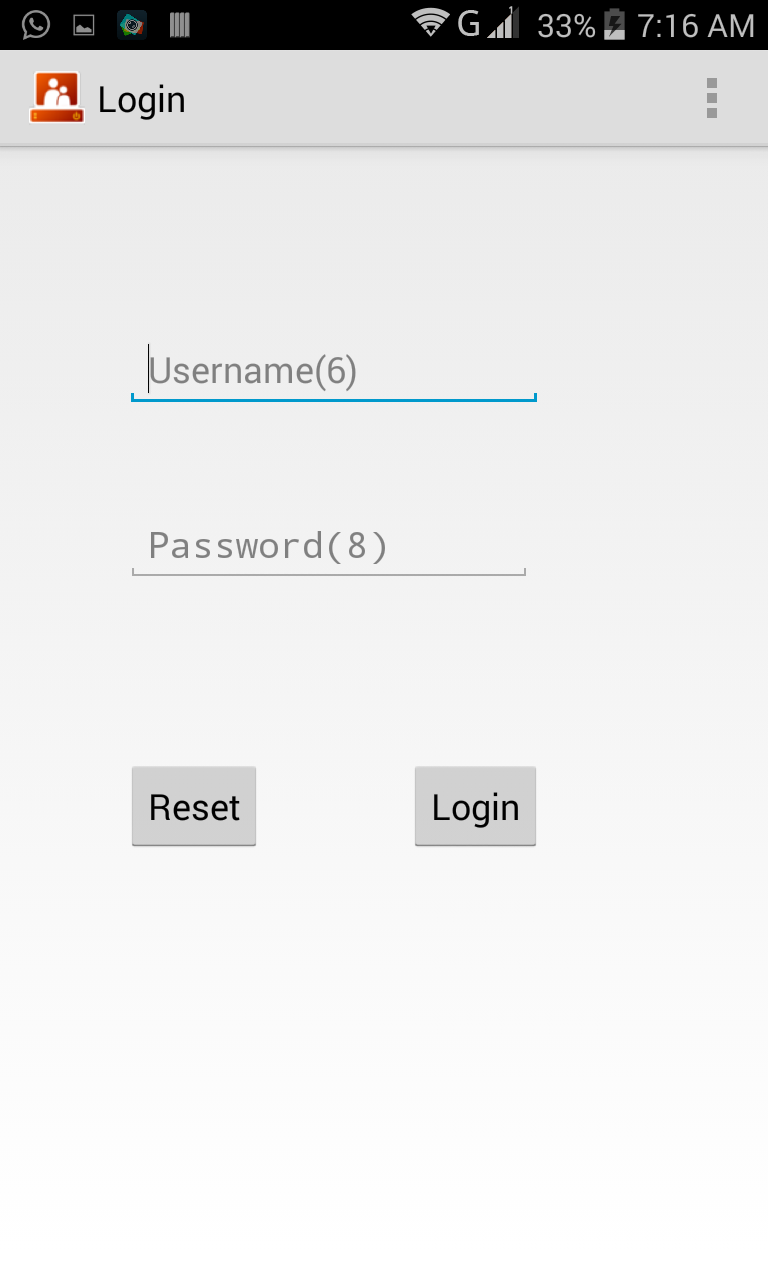
\includegraphics[width=4cm]{login.png}
    \label{fig:pc control system}
\end{figure}
   \end{itemize}
 \end{frame} 
 
 \begin{frame}{DESIGN(Cont...)}  
   \begin{itemize}
  	\item Connection Window 
 	 \begin{figure}[ht!]
     \centering
    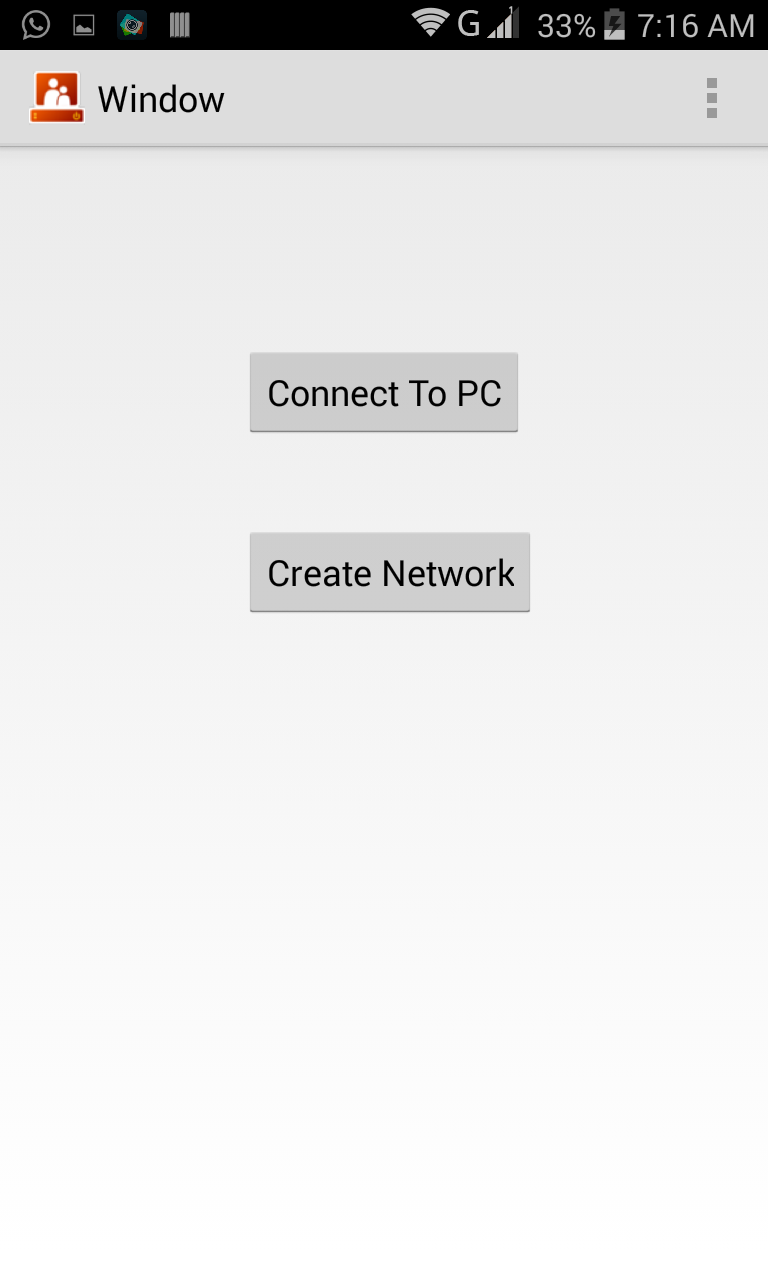
\includegraphics[width=4cm]{window.png}
    \label{fig:pc control home}
\end{figure}
   \end{itemize}
 \end{frame} 
 
 \begin{frame}{DESIGN(Cont...)}  
   \begin{itemize}
  	\item System Configuration
 	 \begin{figure}[ht!]
     \centering
    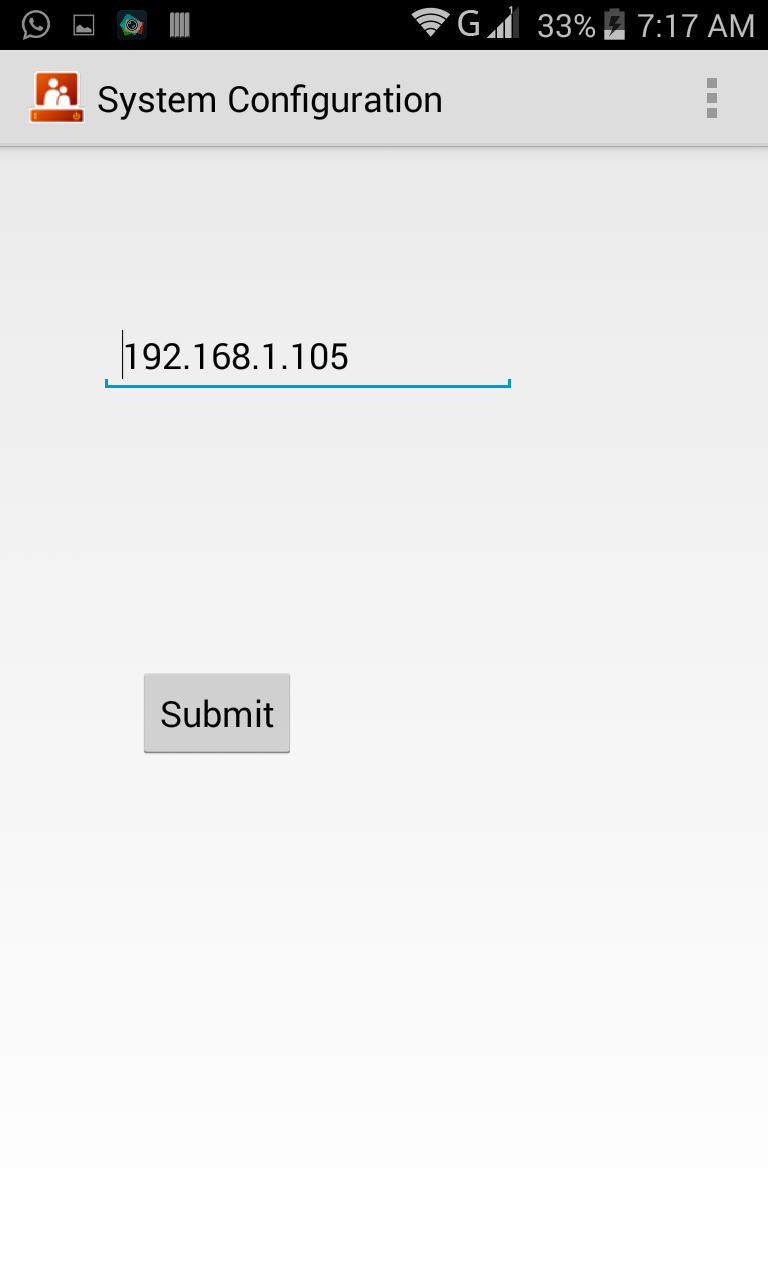
\includegraphics[width=4cm]{system.png}
    \label{fig:pc control desktop}
\end{figure}
   \end{itemize}
 \end{frame} 
 

\begin{frame}{DESIGN(Cont...)}  
   \begin{itemize}
  	\item Home Options
 	 \begin{figure}[ht!]
     \centering
    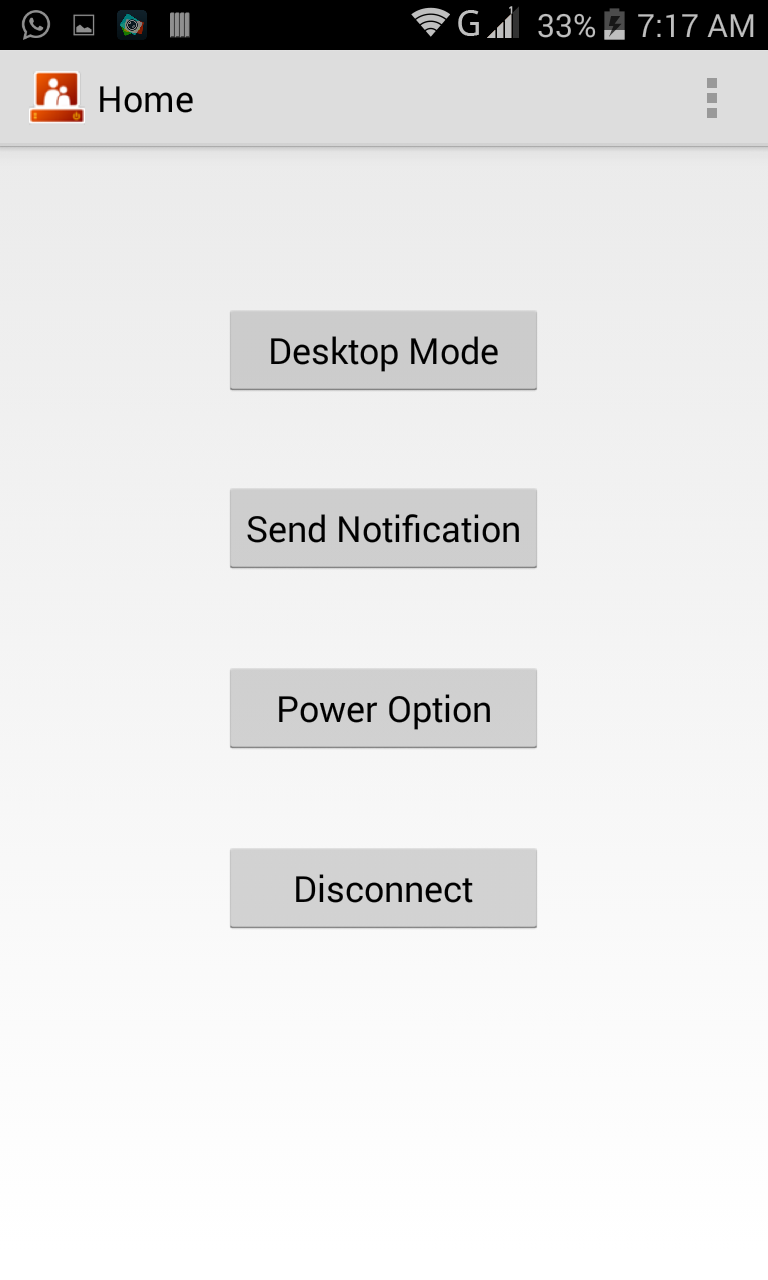
\includegraphics[width=4cm]{home.png}
    \label{fig:pc control desktop}
\end{figure}
   \end{itemize}
 \end{frame} 
 
\begin{frame}{DESIGN(Cont...)}  
   \begin{itemize}
  	\item Remote Desktop Access
 	 \begin{figure}[ht!]
     \centering
    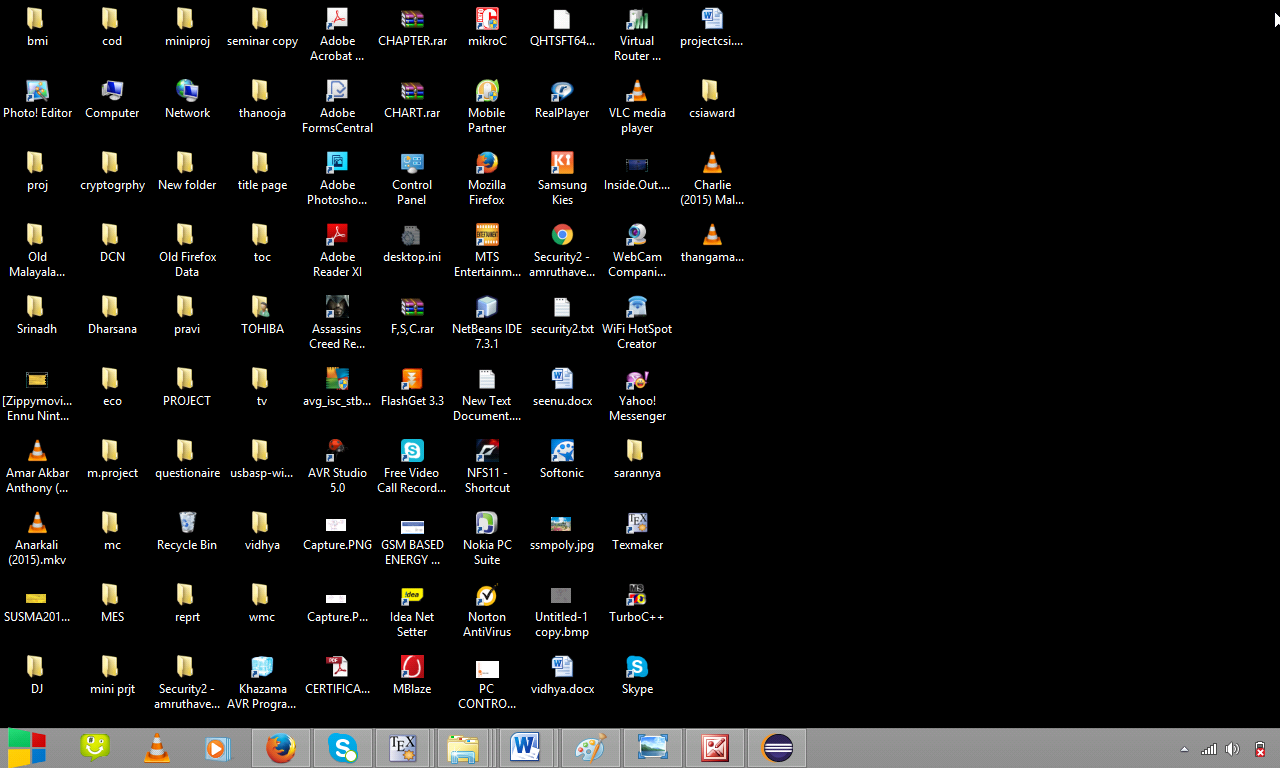
\includegraphics[width=4cm]{desk.png}
    \label{fig:pc control desktop}
\end{figure}
   \end{itemize}
 \end{frame} 
 
\begin{frame}{DESIGN(Cont...)}  
   \begin{itemize}
  	\item Send Notification
 	 \begin{figure}[ht!]
     \centering
    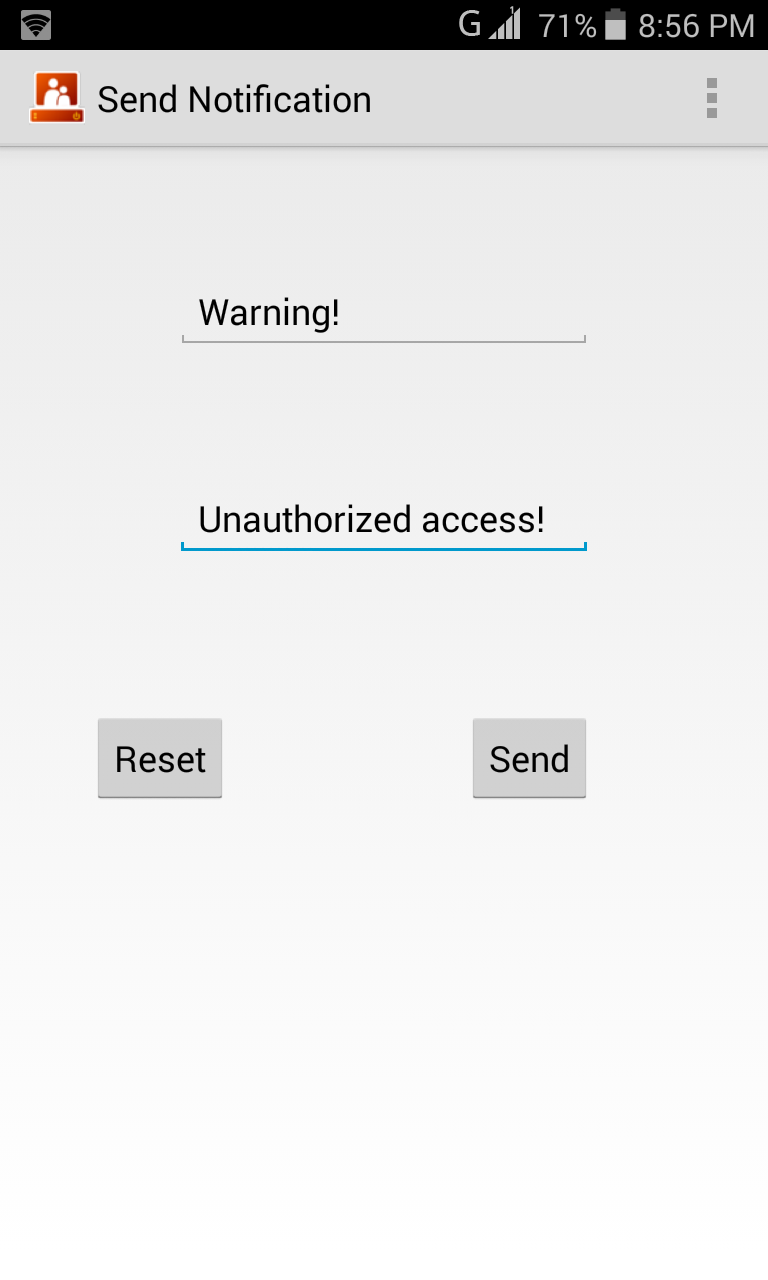
\includegraphics[width=4cm]{message.png}
    \label{fig:pc control desktop}
\end{figure}
   \end{itemize}
 \end{frame} 
 
\begin{frame}{DESIGN(Cont...)}  
   \begin{itemize}
  	\item Power Options
 	 \begin{figure}[ht!]
     \centering
    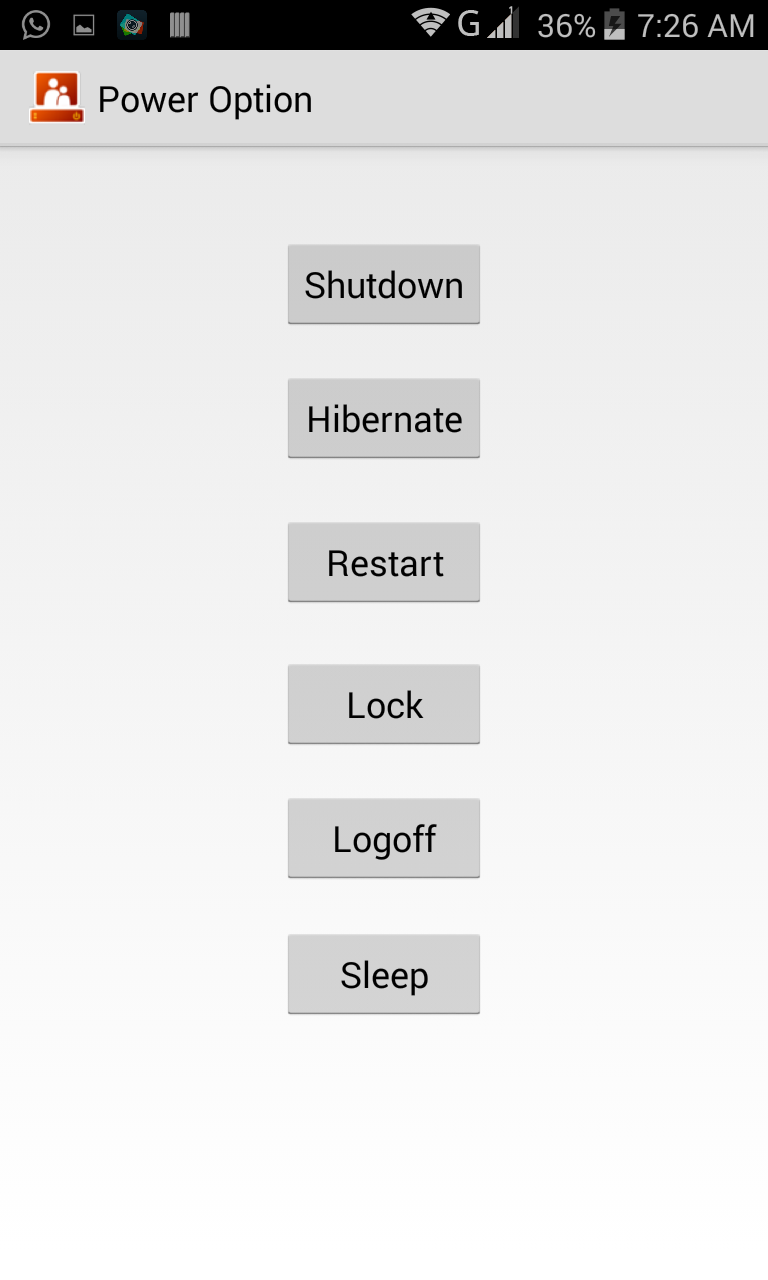
\includegraphics[width=4cm]{power.png}
    \label{fig:pc control desktop}
\end{figure}
   \end{itemize}
 \end{frame} 
 
\begin{frame}{DESIGN(Cont...)}  
   \begin{itemize}
  	\item Message Notification
 	 \begin{figure}[ht!]
     \centering
    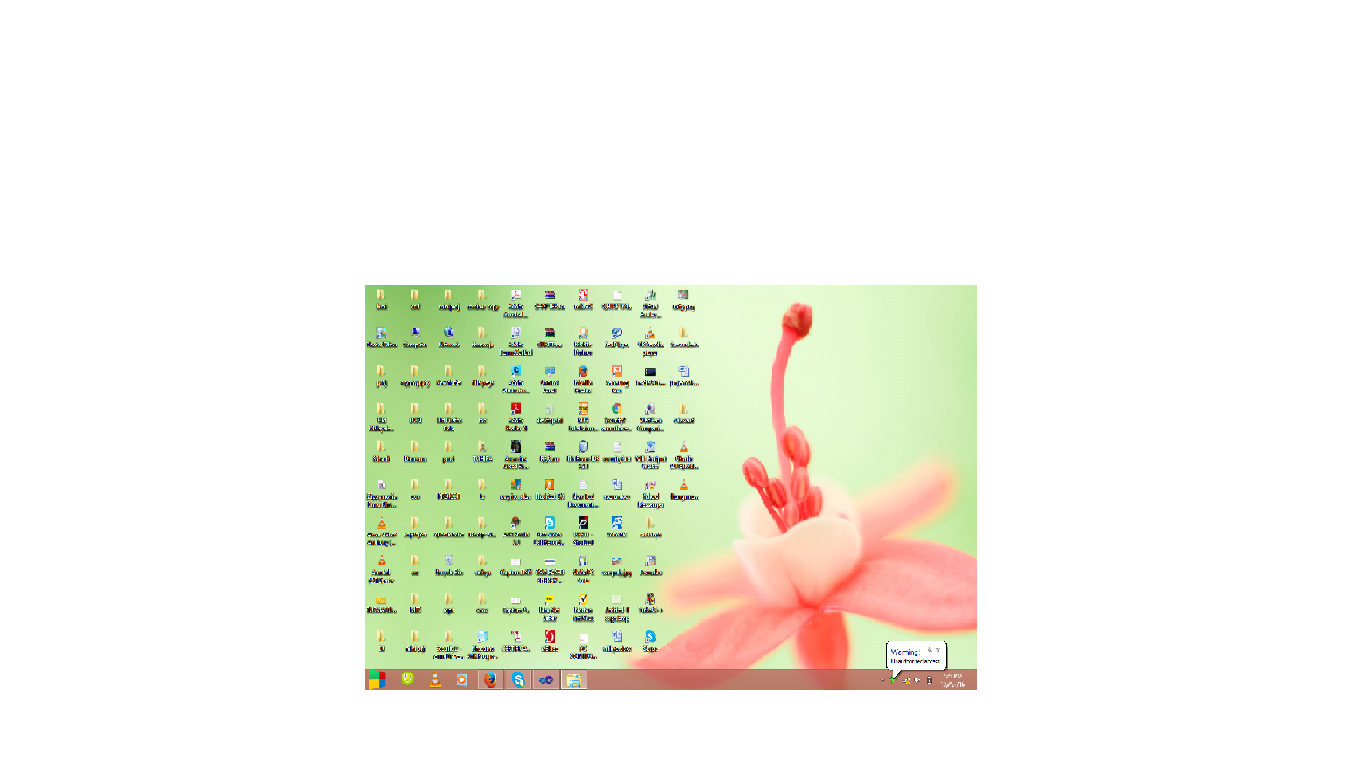
\includegraphics[width=4cm]{notify.png}
    \label{fig:pc control desktop}
\end{figure}
   \end{itemize}
 \end{frame} 
 


 \subsection{CONCLUSION AND FUTURE WORK}
\begin{frame}{CONCLUSION AND FUTURE WORK}
\begin{itemize}
\item Software enables you to get a view of the remote machine desktop.
\item It can be used to perform remote system control and administration tasks.
\item Modify the application software to multi-user environment.
\item Attach documentation and help links.
\end{itemize}

\end{frame}

 \subsection{REFERENCES}
  \begin{frame}{REFERENCE}
  \begin{itemize}
  \item http://www.iis.net/learn/install/installing-iis
  \item http://tightvnc.com
  \item http://www.vogella.com/tutorials/Eclipse/article.html
  \item http://www.vbtutor.net/index.com
  \end{itemize}
  \end{frame}
  
  
 
\begin{frame}
\centerline{Thank You}
\end{frame}
% End of slides

\end{document}

